% Foliensatz: "AFu-Kurs nach DJ4UF" von DK0TU, Amateurfunkgruppe der TU Berlin
% Lizenz: CC BY-NC-SA 3.0 de (http://creativecommons.org/licenses/by-nc-sa/3.0/de/)
% Autoren: Felix Baum <baum@campus.tu-berlin.de>

\documentclass[aspectratio=169]{beamer}

\usepackage[ngerman]{babel} % deutsche Worttrennung etc.
\usepackage[utf8]{inputenc} % UTF8 Text

\usepackage[super, comma, numbers, square, sort]{natbib}

\usepackage{hyperref}       % Hyperref Package für bessere Referenzen (todo)
\hypersetup{
	colorlinks=false,       %   false: boxed links; true: colored links
    %linkcolor=white,       %   color of internal links (change box color with linkbordercolor)
    citecolor=red,          %   color of links to bibliography
    filecolor=white,        %   color of file links
    urlcolor=blue           %   color of external links
}

\usepackage{multirow}
\usepackage{wasysym}  % Math Symbols like \permil
%\usepackage{colortbl}
%\usepackage{subscript}
%\usepackage{caption}
%\usepackage{setspace}
%\usepackage{xcolor}        % benutze CodeListe

% Footnote
%\usepackage{hanging}
%
%\setbeamertemplate{footnote}{%
%  \hangpara{2em}{1}%
%  \makebox[2em][l]{\insertfootnotemark}\footnotesize\insertfootnotetext\par%
%}


%\usepackage{pgf}
%\usepackage{tikz}
%\usetikzlibrary{arrows,automata}
%\usetikzlibrary{positioning}
%
%\tikzset{
%    state/.style={
%           rectangle,
%           rounded corners,
%           draw=black, very thick,
%           minimum height=2em,
%           minimum width=2pt,
%           inner sep=2pt,
%           text centered,
%           },
%}

%\usepackage{listings}
%\lstset{basicstyle=\small, numberstyle=\tiny, extendedchars=true, numbers=left, numbersep=5pt}
%\lstset{showtabs=false, showspaces=false, showstringspaces=false}
%%\lstset{backgroundcolor=\color{white!75!lightgray}, , frame=single}
%%\lstset{backgroundcolor=\color{white}}
%%\lstset{backgroundcolor=none}
%\lstset{keywordstyle=\color{blue!50!gray},  identifierstyle=\color{black}}
%\lstset{commentstyle=\color{green!50!gray}, stringstyle=\color{red!50!gray}}
%\lstset{language=C, fontadjust=true, tabsize=2, breaklines=true}
%\lstset{backgroundcolor=\color{white!75!lightgray}, caption=\lstname, frame=single}
%\lstset{emphstyle=\color{black}\fbox}
%
%% Keine "Listing:"-Caption
%\captionsetup{labelformat=empty,labelsep=none}
%
%% für mathematische Umgebungen
%\usepackage{amsmath,amsfonts,amssymb}
%
%\lstdefinestyle{Bash}{
%language=Bash,
%frame=single,
%rulecolor=\color{black},
%backgroundcolor=\color{gray!50},
%keywordstyle=\color{black},
%identifierstyle=,
%commentstyle=\color{black},
%stringstyle=\color{magenta!65!white},
%showstringspaces=false,
%basicstyle=\footnotesize\ttfamily\color{black},
%numbers=none,
%breaklines=true,
%captionpos=b
%}

%\usepackage{listings}
%
%\lstdefinestyle{basic}{
%    captionpos=t,%
%    basicstyle=\footnotesize\ttfamily,%
%    numberstyle=\tiny,%
%    numbers=left,%
%    stepnumber=1,%
%    frame=single,%
%    showspaces=false,%
%    showstringspaces=false,%
%    showtabs=false,%
%    %
%    keywordstyle=\color{blue},%
%    identifierstyle=,%
%    commentstyle=\color{gray},%
%    stringstyle=\color{magenta}%
%}



% fließende Boxen haben keinen Abstand
%\fboxsep0mm

% inkludiere Creative Commons Helper
%%%%%%%%%%%%%%%%%%%%%%%%%%%%%%%%%%%%%%%%%%%%%%%%%%%%%%%%%%%%%%%%
%% ccBeamer 0.1, 2007-07-02                                   %%
%% Written by Sebastian Pipping <webmaster@hartwork.org>      %%
%% ---------------------------------------------------------- %%
%% Licensed under Creative Commons Attribution-ShareAlike 3.0 %%
%% http://creativecommons.org/licenses/by-sa/3.0/             %%
%%%%%%%%%%%%%%%%%%%%%%%%%%%%%%%%%%%%%%%%%%%%%%%%%%%%%%%%%%%%%%%%


%% Images
\newcommand{\CcImageBy}[1]{%
	
\includegraphics[scale=#1]{texdata/creative_commons/cc_by_30.pdf}%
}
\newcommand{\CcImageCc}[1]{%
	
\includegraphics[scale=#1]{texdata/creative_commons/cc_cc_30.pdf}%
}
\newcommand{\CcImageDevNations}[1]{%
	
\includegraphics[scale=#1]{texdata/creative_commons/cc_dev_nations_30.pdf}%
}
\newcommand{\CcImageNc}[1]{%
	
\includegraphics[scale=#1]{texdata/creative_commons/cc_nc_30.pdf}%
}
\newcommand{\CcImageNd}[1]{%
	
\includegraphics[scale=#1]{texdata/creative_commons/cc_nd_30.pdf}%
}
\newcommand{\CcImagePd}[1]{%
	
\includegraphics[scale=#1]{texdata/creative_commons/cc_pd_30.pdf}%
}
\newcommand{\CcImageSa}[1]{%
	
\includegraphics[scale=#1]{texdata/creative_commons/cc_sa_30.pdf}%
}
\newcommand{\CcImageSampling}[1]{%
	
\includegraphics[scale=#1]{texdata/creative_commons/cc_sampling_30.pdf}%
}
\newcommand{\CcImageSamplingPlus}[1]{%
	
\includegraphics[scale=#1]{texdata/creative_commons/cc_sampling_plus_30.pdf}%
}


%% Groups
\newcommand{\CcGroupBy}[2]{% zoom, gap
	\CcImageCc{#1}\hspace*{#2}\CcImageBy{#1}%
}
\newcommand{\CcGroupByNc}[2]{% zoom, gap
	\CcImageCc{#1}\hspace*{#2}\CcImageBy{#1}\hspace*{#2}\CcImageNc{#1}%
}
\newcommand{\CcGroupByNcNd}[2]{% zoom, gap
	\CcImageCc{#1}\hspace*{#2}\CcImageBy{#1}\hspace*{#2}\CcImageNc{#1}\hspace*{#2}\CcImageNd{#1}%
}
\newcommand{\CcGroupByNcSa}[2]{% zoom, gap
	\CcImageCc{#1}\hspace*{#2}\CcImageBy{#1}\hspace*{#2}\CcImageNc{#1}\hspace*{#2}\CcImageSa{#1}%
}
\newcommand{\CcGroupByNd}[2]{% zoom, gap
	\CcImageCc{#1}\hspace*{#2}\CcImageBy{#1}\hspace*{#2}\CcImageNd{#1}%
}
\newcommand{\CcGroupBySa}[2]{% zoom, gap
	\CcImageCc{#1}\hspace*{#2}\CcImageBy{#1}\hspace*{#2}\CcImageSa{#1}%
}
\newcommand{\CcGroupDevNations}[2]{% zoom, gap
	\CcImageCc{#1}\hspace*{#2}\CcImageDevNations{#1}%
}
\newcommand{\CcGroupNcSampling}[2]{% zoom, gap
	\CcImageCc{#1}\hspace*{#2}\CcImageNc{#1}\hspace*{#2}\CcImageSampling{#1}%
}
\newcommand{\CcGroupPd}[1]{% zoom
	\CcImagePd{#1}%
}
\newcommand{\CcGroupSampling}[1]{% zoom
	\CcImageSampling{#1}%
}
\newcommand{\CcGroupSamplingPlus}[1]{% zoom
	\CcImageSamplingPlus{#1}%
}


%% Text
\newcommand{\CcLongnameBy}{Attribution}
\newcommand{\CcLongnameByNc}{Attribution-NonCommercial}
\newcommand{\CcLongnameByNcNd}{Attribution-NoDerivs}
\newcommand{\CcLongnameByNcSa}{Attribution-NonCommercial-ShareAlike}
\newcommand{\CcLongnameByNd}{Attribution-NoDerivs}
\newcommand{\CcLongnameBySa}{Attribution-ShareAlike}

\newcommand{\CcNote}[1]{% longname
	This work is licensed under the \textit{Creative Commons #1 3.0 License}.%
}


% generelles Thema auswählen
\usetheme{Goettingen} %Berlin spart ohne Sidebar allerdings angenehm Platz
% AnnArbor | Antibes | Bergen | Berkeley | Berlin | Boadilla | boxes | CambridgeUS | Copenhagen | Darmstadt | default | Dresden | Frankfurt | Goettingen | Hannover | Ilmenau | JuanLesPins | Luebeck | Madrid | Malmoe | Marburg | Montpellier | PaloAlto | Pittsburgh | Rochester | Singapore | Szeged | Warsaw

% Farben wählen
\usecolortheme{beetle}
% beaver | beetle | crane | default | dolphin | dove | fly | lily | orchid | rose | seagull | seahorse | sidebartab | structure | whale | wolverine

% Setze alle Farben auf Grau und Weiß
%\definecolor{craneorange}{RGB}{64,64,64}
%\definecolor{craneblue}{RGB}{255,255,255}

% Schriftart wählen
\usefonttheme{default}
% default | professionalfonts | serif | structurebold | structureitalicserif | structuresmallcapsserif

% Innere Themen(Kopf-, Fuß-, Sidebar usw)
%\useinnertheme{default}
\useinnertheme{circles}
% default | inmargin | rectangles | rounded | circles

% Äußere Themen (Anordnung der inneren, grenzen der Folien etc.)
\useoutertheme{infolines}
% default | infolines | miniframes | shadow | sidebar | smoothbars | smoothtree | split | tree

% Deaktiviere Navigations-Symbole ({} -> leer)
\setbeamertemplate{navigation symbols}{}
%\setbeamertemplate{navigation symbols}{\large \ifnum \insertframenumber <10 0\fi\insertframenumber/\inserttotalframenumber\vspace*{0.2ex}}

% Zeige ein Hintergrundbild
\setbeamertemplate{background canvas}{
        \hspace*{-2.0cm}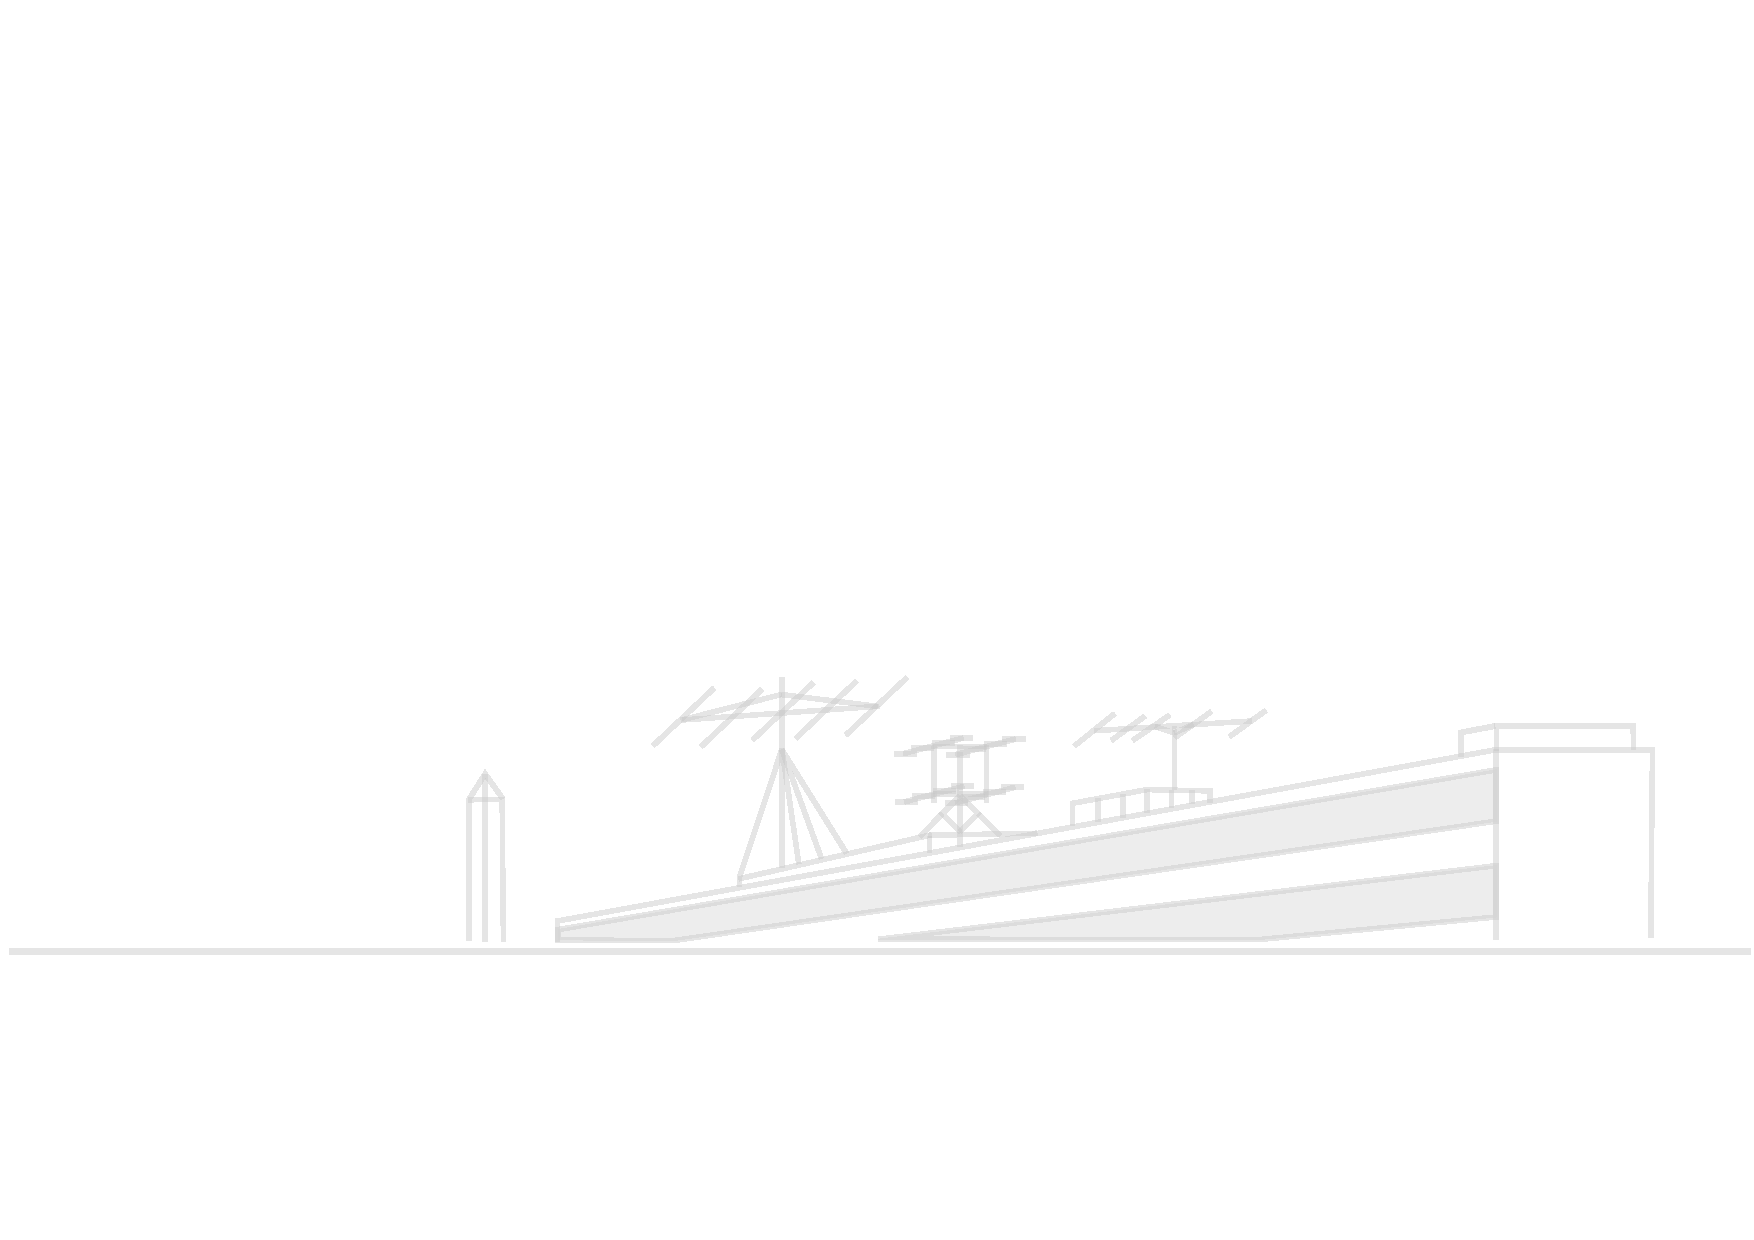
\includegraphics[width=17.8cm]{texdata/dk0tu_rooftop_background.pdf}
}

% Foliennummer einfügen
\setbeamertemplate{footline}[frame number]
%\setbeamertemplate{footline}{}

% Ändere das Zeichen vor jedem item
%\setbeamertemplate{itemize item}{\color{craneorange}$\blacktriangleright$}
%\setbeamertemplate{itemize subitem}{\color{craneorange}$\triangleright$}
%\setbeamertemplate{itemize subsubitem}{\color{craneorange}$\blacktriangleright$}

% Ändert die Blöcke 
\setbeamertemplate{blocks}[rounded][shadow=true]
% default | rounded [shadow=true|false]

%
% Eigene Kommandos
%

% Hack to get natbib and beamer working together. "The beamer user guide suggests
% that only the manual bibliography entry approach is supported"
% on some system it works out of the box, sometimes you need the hack :-(
% so check it --dl7bst
\ifdefined\newblock
    \relax
\else
    \newcommand{\newblock}{}
\fi

% \includedia command to generate png out of a dia file
% NEEDS installed dia and pdflatex option --shell-escape
\newcommand{\includedia}[1]{
    \immediate\write18{/usr/bin/dia #1.dia -e #1_diatmp.png -t png}
}

% RICHIG GROSSER FONT!
\newfont{\bigfont}{cmr10 at 144pt}
\newfont{\smallfont}{cmr10 at 8pt}

% Römische Ziffern
\makeatletter
\newcommand{\rmnum}[1]{\romannumeral #1}
\newcommand{\Rmnum}[1]{\expandafter\@slowromancap\romannumeral #1@}
\makeatother

% Schwarze Überschrift
%\setbeamercolor{frametitle}{fg=black}
%\setbeamercolor{title}{fg=black}

% Item- und Box-Farben
\definecolor{deepBlue}{HTML}{000066}
\setbeamercolor{itemize item}{fg=deepBlue}
\setbeamercolor{itemize subitem}{fg=deepBlue}
\setbeamercolor{description item}{fg=deepBlue}
\setbeamercolor{block title}{fg=deepBlue!100, bg=blue!15}
\setbeamercolor{block body}{fg=black, bg=blue!5}
\setbeamercolor{block title alerted}{fg=deepBlue, bg=red!75}
\setbeamercolor{block body alerted}{fg=black, bg=red!15}
\setbeamercolor*{block title example}{fg=blue!50, bg=blue!10}
\setbeamercolor*{block body example}{fg= blue, bg=blue!5}

%\setbeamercolor{section in head/foot}{parent=palette primary}
%\setbeamercolor{subsection in head/foot}{parent=palette secondary}
%\setbeamercolor{sidebar}{fg=darkblue,bg=yellow!90!orange}
%\setbeamercolor{title in sidebar}{fg=darkblue}
%\setbeamercolor{author in sidebar}{fg=darkblue}
%\setbeamercolor{section in sidebar}{fg=darkblue!10!black}
%\setbeamercolor{subsection in sidebar}{fg=darkblue!50!black}

% Titlepage Infos
\title{AFu-Kurs nach DJ4UF}
\author[DKØTU]{DKØTU\\ \footnotesize{Amateurfunkgruppe der TU Berlin}}
\institute[DKØTU]{\url{http://www.dk0tu.de} }

% PDF-Eigenschaften
\subject{DK0TU-Amateurfunkkurs nach DJ4UF}
\keywords{Amateurfunk Kurs HAM Radio Course CC-BY-NC-SA OpenSource TU Berlin DK0TU}

\subtitle{Technik 09: \\
           Die Wellenausbreitung \\[2em]}
\date{Stand 22.11.2014}
 \begin{document}

\begin{frame}
    \titlepage
    \vfill
    \begin{center}
        \ccbyncsaeu\\
        {\tiny This work is licensed under the \em{Creative Commons Attribution-NonCommercial-ShareAlike 3.0 License}.}\\[0.5ex]
         \tiny Amateurfunkgruppe der Technische Universität Berlin (AfuTUB), DKØTU
         %\includegraphics[scale=0.5]{img/DK0TU_Logo.pdf}
    \end{center}
\end{frame}


%fixme Referenzen/Fußnoten-Systematik vereinheitlichen

\section*{Einleitung}

\begin{frame}
    \frametitle{Wie kommen die Wellen um die Welt?}
    \begin{center}
        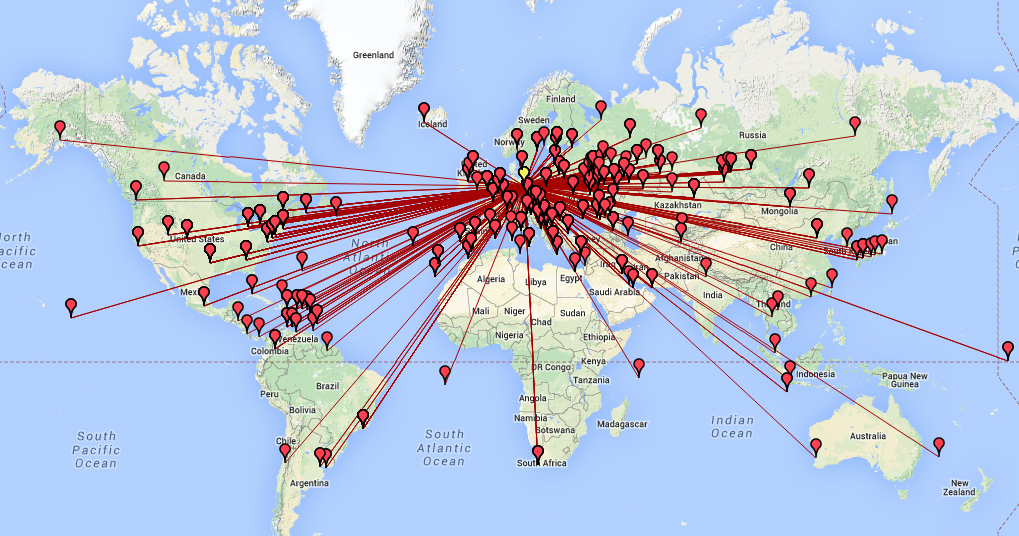
\includegraphics[width=1\textwidth]{e09/cqww-kontakte.png}
        \footnote{\tiny Funkkontakte beim CQWW-SSB 2014 von DK0TU}
    \end{center}
\end{frame}

\begin{frame}
    \frametitle{Raum und Bodenwelle}
	\begin{center}
        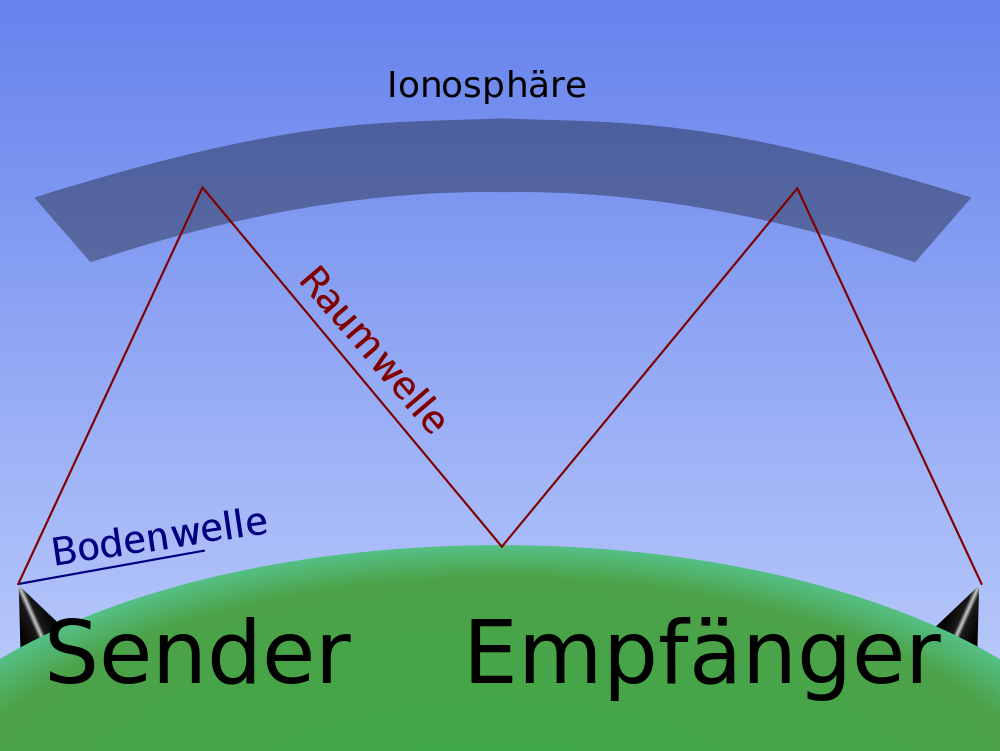
\includegraphics[width=.8\textwidth]{e09/Ionospheric_reflectionpng.png}
         \footnote{\tiny \url{https://commons.wikimedia.org/wiki/File:Ionospheric_reflection-de.svg}}
    \end{center}
\end{frame}

\begin{frame}
    \frametitle{Raum und Bodenwelle}
	\begin{itemize}
        \item Bodenwelle
			\begin{itemize}
				\item Folgt der Erdkrümmung
       		 	\item Stark vorhanden bei Langwelle und Mittelwelle
        		\item Viele Verluste durch Berge, Wälder und Städte
    		\end{itemize}
        \item Raumwelle
			\begin{itemize}
       		 	\item Meist genutzt bei Kurzwelle (Manchmal auch UHF, VHF)
        		\item Reflektion an der Ionosphäre 
        		\item Nicht Zuverlässig für Überreichweiten
    		\end{itemize}
    \end{itemize}
\end{frame}

\section*{Bodenwelle}
\begin{frame}
    \frametitle{Bodenwelle}
	\begin{itemize}
				\item Bei LF über $400km$
       		 	\item $80m$ Wellemlänge ($3.5MHz$)  - $150km$ Reichweite
        		\item $10m$ Wellenlänge ($28MHz$) - $30km$ Reichweite
        		\item Reichweite hängt auch stark vom Untergrund ab.
    \end{itemize}
\end{frame}

\begin{frame}
    \frametitle{Prüfungsfrage}

    \begin{center}
    \begin{tabular}{l||l}\hline
        TI203 & Welche der folgenden Aussagen trifft für KW-Funk- \\
         " "  & verbindungen zu, die über Bodenwellen erfolgen? \\ 
         " "  & Die Bodenwelle folgt der Erdkrümmung und ...\\\hline\hline
         A 	  & geht nicht über den geografischen Horizont hinaus. \\
         " "  & Sie wird in niedrigeren Frequenzbereichen stärker \\ 
         " "  & gedämpft als in höheren Frequenzbereichen.\\\hline
         B 	  & geht über den geografischen Horizont hinaus. Sie \\
         " "  & wird in höheren Frequenzbereichen stärker gedämpft \\ 
         " "  & als in niedrigeren Frequenzbereichen.\\\hline
         C	  & geht über den geografischen Horizont hinaus. Sie \\
         " "  & wird in niedrigeren Frequenzbereichen stärker \\ 
         " "  & gedämpft als in höheren Frequenzbereichen.\\\hline
         D 	  & geht nicht über den geografischen Horizont hinaus. \\
         " "  & Sie wird in höheren Frequenzbereichen stärker \\ 
         " "  & gedämpft als in niedrigeren Frequenzbereichen.\\\hline
    \end{tabular}
 	\end{center}
\end{frame}

\begin{frame}
    \frametitle{Prüfungsfrage}

    \begin{center}
    \begin{tabular}{l||l}\hline
        TI203 & Welche der folgenden Aussagen trifft für KW-Funk- \\
         " "  & verbindungen zu, die über Bodenwellen erfolgen? \\ 
         " "  & Die Bodenwelle folgt der Erdkrümmung und ...\\\hline\hline
         " " 	  & geht nicht über den geografischen Horizont hinaus. \\
         " "  & Sie wird in niedrigeren Frequenzbereichen stärker \\ 
         " "  & gedämpft als in höheren Frequenzbereichen.\\\hline
         " " 	  & geht über den geografischen Horizont hinaus. Sie \\
         x  & wird in höheren Frequenzbereichen stärker gedämpft \\ 
         " "  & als in niedrigeren Frequenzbereichen.\\\hline
         " "	  & geht über den geografischen Horizont hinaus. Sie \\
         " "  & wird in niedrigeren Frequenzbereichen stärker \\ 
         " "  & gedämpft als in höheren Frequenzbereichen.\\\hline
         " " 	  & geht nicht über den geografischen Horizont hinaus. \\
         " "  & Sie wird in höheren Frequenzbereichen stärker \\ 
         " "  & gedämpft als in niedrigeren Frequenzbereichen.\\\hline
    \end{tabular}
 	\end{center}
\end{frame}

\section*{Raumwelle}
    
\begin{frame}
    \frametitle{Raumwelle}
	\begin{center}
        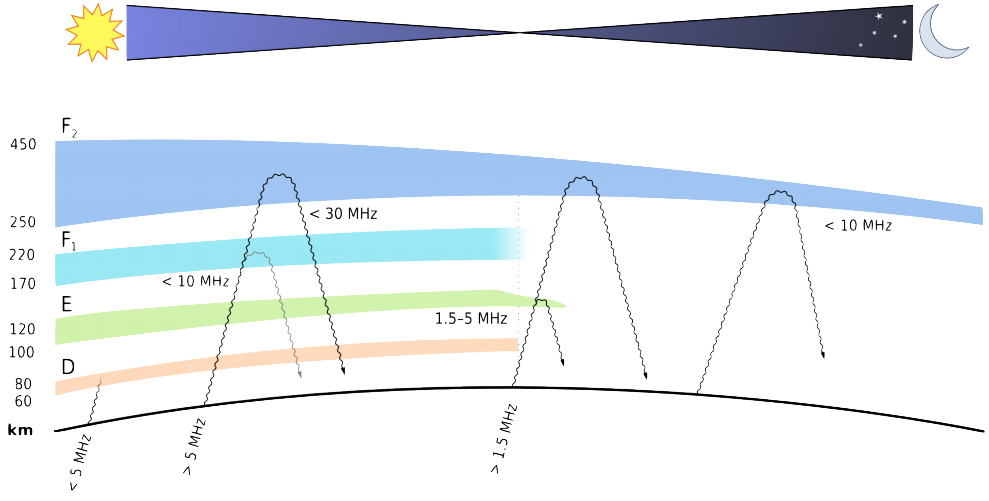
\includegraphics[width=.9\textwidth]{e09/schichten_behelf_43.png}
        \footnote{\tiny Amateurfunkbehelf s.43 \url{http://ham.granjow.net/builds/Amateurfunkbehelf.pdf}}
    \end{center}
\end{frame}

\begin{frame}
    \frametitle{Sonnenflecken Zyklus}
    \begin{itemize}
    			\item Bei Sonneneinstrahlung werden Moleküle in der Ionosphäre durch EUV-Strahlung ionisiert
				\item Maximum ca alle 11 Jahre
       		 	\item HF Frequenzen ab ca $20MHz$ sind bei einem Minimum nicht verwendbar
       		 	\item Bei einem Maximum quasi Täglich DX-Verbindungen mit weniger als $10W$ machbar 
        		\item Nächstes Maximum vermutlich 2022
    \end{itemize}
	\begin{center}
        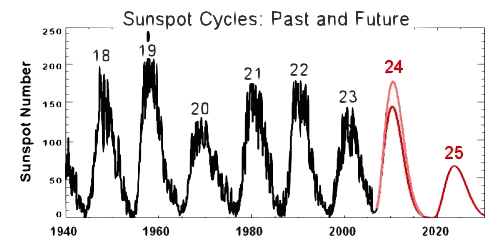
\includegraphics[width=0.8\textwidth]{e09/Predictions_sunspot.png}
        \footnote{\tiny By Scientific data, based on prediction by David Hathaway, Public domain, via Wikimedia Commons \url{https://commons.wikimedia.org/wiki/File_3APredictions3_strip.jpg}} %\url{https://commons.wikimedia.org/wiki/File%3APredictions3_strip.jpg}
    \end{center}
\end{frame}

\begin{frame}
    \frametitle{D-Schicht}
    \begin{itemize}
    			\item Tagsüber und verschwindet nach Sonnenuntergang sehr schnell
				\item Dämpft Frequenzen unter $5MHz$ (160m und 80m unbenutzbar)
       		 	\item HF Frequenzen ab ca $20MHz$ sind bei einem Minimum nicht verwendbar
       		 	\item Bei hoher Sonnenaktivität Möbel-Dellinger-Effekt (Kurzzeitig ganzes KW-Band unbenutzbar)
    \end{itemize}
    \begin{center}
        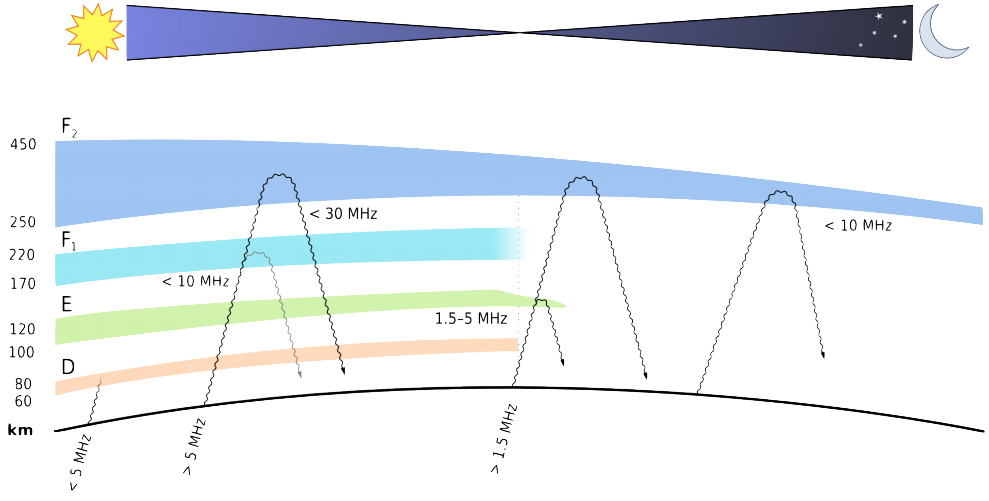
\includegraphics[width=.6\textwidth]{e09/schichten_behelf_43.png}
        \footnote{\tiny Amateurfunkbehelf s.43 \url{http://ham.granjow.net/builds/Amateurfunkbehelf.pdf}}
    \end{center}
\end{frame}

\begin{frame}
    \frametitle{E-Schicht}
    \begin{itemize}
    			\item Tagsüber
				\item Reflektiert HF-Bänder 10m, 6m
       		 	\item Refelktiert gelegendlich 2m (Sporedic-E) \footnote{\tiny \url{https://www.youtube.com/watch?v=xSWTkuSekhE}}
       		 	\item (Short Skip)mit sehr starken Signalen zwischen 750 und 2200 km (Short-Skip)
    \end{itemize}
    \begin{center}
        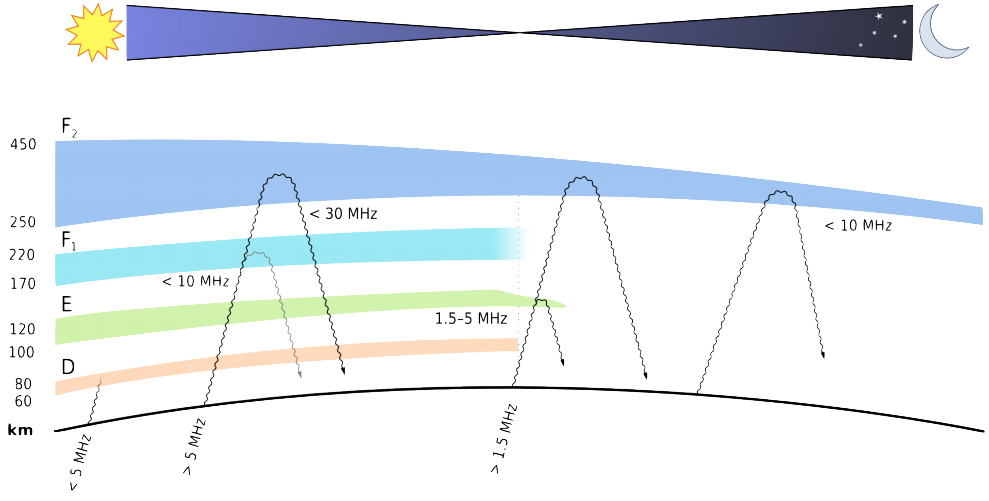
\includegraphics[width=.75\textwidth]{e09/schichten_behelf_43.png}
        \footnote{\tiny Amateurfunkbehelf s.43 \url{http://ham.granjow.net/builds/Amateurfunkbehelf.pdf}}
    \end{center}
\end{frame}

\begin{frame}
    \frametitle{F-Schichten}
    \begin{itemize}
    			\item F1 und F2 Schicht
				\item F2 Schicht besteht auch Nachts (langsame Rekombination)
       		 	\item Wichtigstens da beständigste Schichten für KW
       		 	\item (Short Skip)mit sehr starken Signalen zwischen 750 und 2200 km (Short-Skip)
    \end{itemize}
	\begin{center}
        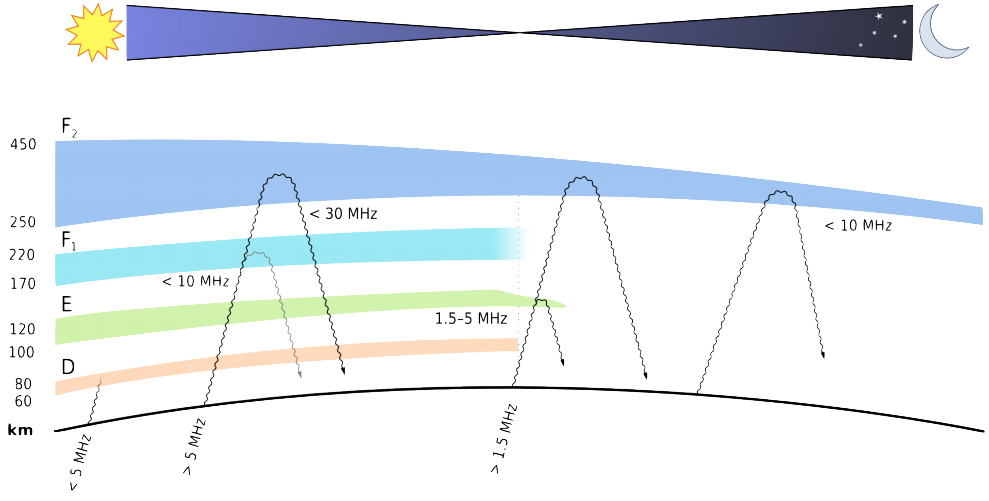
\includegraphics[width=.75\textwidth]{e09/schichten_behelf_43.png}
        \footnote{\tiny Amateurfunkbehelf s.43 \url{http://ham.granjow.net/builds/Amateurfunkbehelf.pdf}}
    \end{center}
\end{frame}

\section*{Besonderes}

\begin{frame}
    \frametitle{Sonstiges}
    \begin{itemize}
    			\item MUF: maximum usable frequency
				\item Tote Zone
       		 	\item Fading
       		 	\item Grey Line
    \end{itemize}
\end{frame}

\begin{frame}
    \frametitle{Aurora}
	\begin{center}
        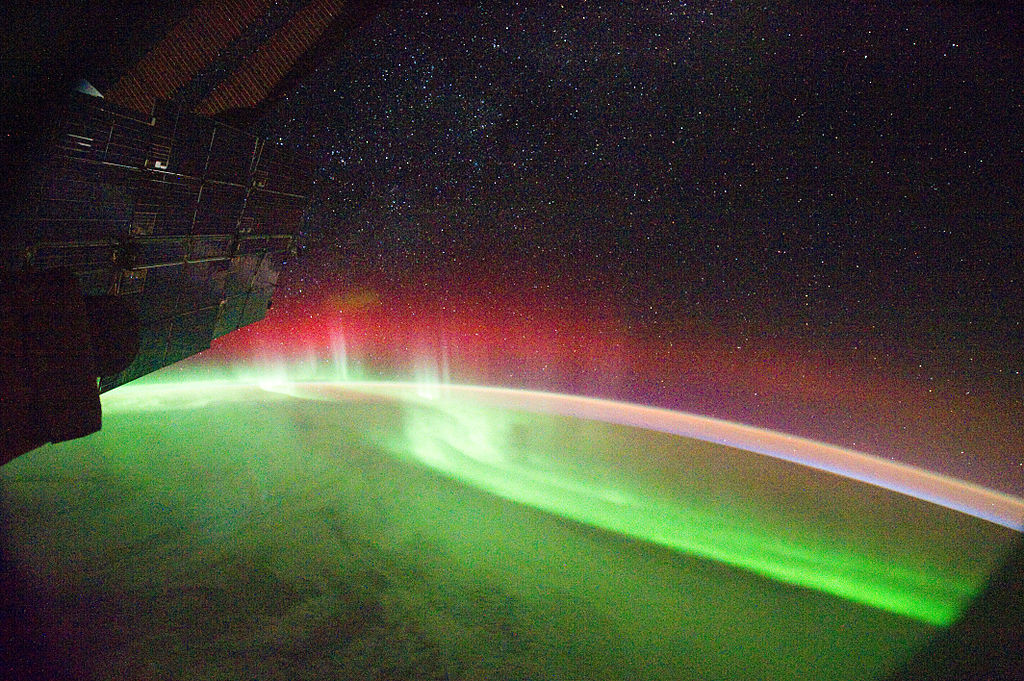
\includegraphics[width=1\textwidth]{e09/Aurora_Seen_From_Space_by_NASA.jpg}
        \footnote{\tiny \url{https://commons.wikimedia.org/wiki/File:Aurora_Seen_From_Space_by_NASA.jpg}}
    \end{center}
\end{frame}

\begin{frame}
    \frametitle{Troposphärische Überreichweiten}
    \begin{itemize}
    			\item Beugt UKW (dadurch Überreichweite)
				\item bekannt als Tropo da nicht Ionosphäre sondern Troposphäre (15km höhe)
       		 	\item Kalte Luft unten, Warme Luft oben sorgt für Brechnung der UKW Wellen
       		 	\item Entfernungen bis ca 700km
    \end{itemize}
    	\begin{center}
        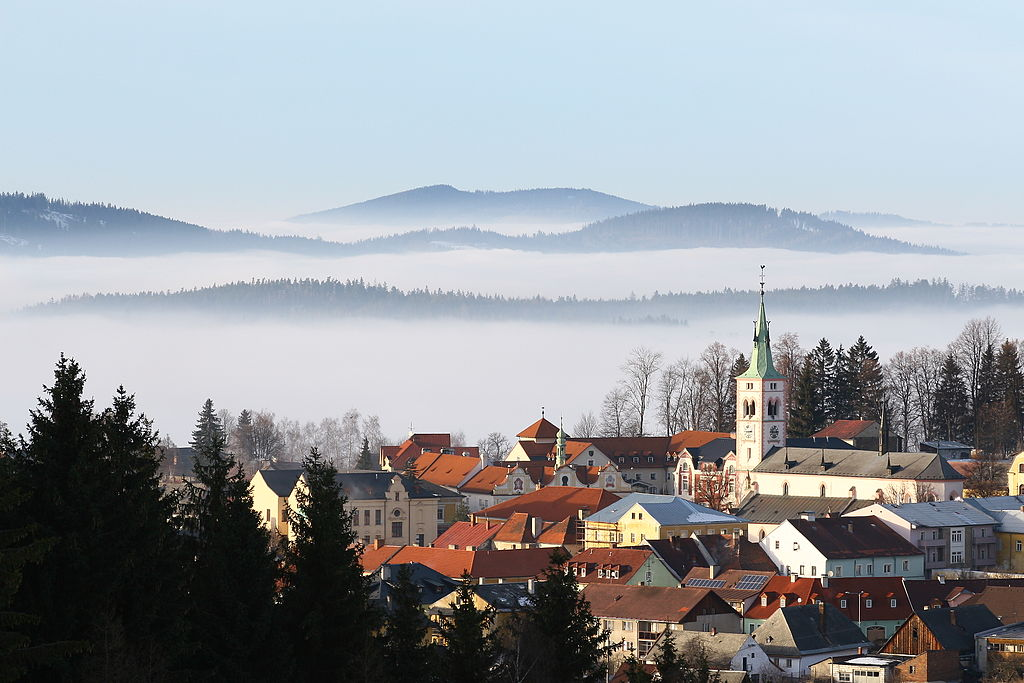
\includegraphics[width=.65\textwidth]{e09/tropo.jpg}
        \footnote{\tiny by Adam Hauner via Wikimedia}
    \end{center}
\end{frame}

\begin{frame}
    \frametitle{Prüfungsfrage}

    \begin{center}
    \begin{tabular}{l||l}\hline
        TI101 & Welche ionosphärischen Schichten bestimmen \\
         " "  & die Wellenausbreitung am Tage? \\\hline\hline
         A 	  & Die E- und D-Schicht \\\hline
         B 	  & Die F1- und F2-Schicht \\\hline
         C	  & Die E- und F-Schicht \\\hline
         D 	  & Die D-, E-, F1- und F2-Schicht\\\hline
    \end{tabular}
 	\end{center}
\end{frame}

\begin{frame}
    \frametitle{Prüfungsfrage}

    \begin{center}
    \begin{tabular}{l||l}\hline
        TI101 & Welche ionosphärischen Schichten bestimmen \\
         " "  & die Wellenausbreitung am Tage? \\\hline\hline
         " " 	  & Die E- und D-Schicht \\\hline
         " " 	  & Die F1- und F2-Schicht \\\hline
         " "	  & Die E- und F-Schicht \\\hline
         X 	  & Die D-, E-, F1- und F2-Schicht\\\hline
    \end{tabular}
 	\end{center}
\end{frame}

\begin{frame}
    \frametitle{Prüfungsfrage}

    \begin{center}
    \begin{tabular}{l||l}\hline
        TI102 & Welche ionosphärischen Schichten bestimmen \\
         " "  & die Wellenausbreitung in der Nacht? \\\hline\hline
         A 	  & Die D-, E- und F2-Schicht \\\hline
         B 	  & Die F2-Schichtt \\\hline
         C	  & Die F1- und F2-Schicht \\\hline
         D 	  & Die D- und E-Schicht\\\hline
    \end{tabular}
 	\end{center}
\end{frame}

\begin{frame}
    \frametitle{Prüfungsfrage}

    \begin{center}
    \begin{tabular}{l||l}\hline
        TI102 & Welche ionosphärischen Schichten bestimmen \\
         " "  & die Wellenausbreitung in der Nacht? \\\hline\hline
         " " 	  & Die D-, E- und F2-Schicht \\\hline
         X 	  & Die F2-Schichtt \\\hline
         " "	  & Die F1- und F2-Schicht \\\hline
         " " 	  & Die D- und E-Schicht\\\hline
    \end{tabular}
 	\end{center}
\end{frame}


\section*{Referenzen}

\begin{frame}
    \frametitle{Referenzen/Links}
    
    \footnotesize
    \begin{itemize}
        \item Moltrecht E 09: \\
              \url{http://www.dj4uf.de/lehrg/e09/e09.html}
        \item Aurora (Youtube): \\
              \url{https://www.youtube.com/watch?v=izYiDDt6d8s}
        \item Spradic E QSO \\
              \url{http://www.dk0tu.de/blog/2012/11/27_Sporadic-E_QSO_mit_Spanien/}
    \end{itemize}

\end{frame}

% Hier könnte noch eine Kontaktfolie stehen

\end{document}

